\chapter{Introduction} \label{ch:introduction}
Anthropogenic emissions of nitrogen oxides ($\chem{NO_x}$), carbon monoxide (\chem{CO}), \acrfull{voc} and methane ($\chem{CH_4}$) causes production of ozone in the troposphere (\cite{SeinfeldSpyros}). Several studies indicate a significant increase in tropospheric ozone concentrations since pre-industrial times, especially in the \acrfull{nh} and the Arctic (eg. \cite{WangJacob1998}, \cite{Shindell2007}, \cite{Parrish2014}, \cite{AMAP2015}). A study performed by \cite{ZIEMKE2019} performed by combining satellite measurements and model results to find ozone trends between 1979-2016 finds large positive trends in tropospheric column ozone in the \acrshort{nh} particularly extending from the India to South East Asia and further eastward over the Pacific ocean. Analysis of \chem{NO} emissions in the simulated period indicated that the increase in in pollution in the region is consistent with the measured trends in tropospheric ozone.  

\medskip

Ozone is a powerful greenhouse gas in terms of \acrfull{rf}, both in the stratosphere and troposphere. The estimated \acrshort{rf} due to tropospheric ozone was reported by The \acrfull{ipcc} as 0.40$\pm$0.20Wm$^{-2}$ (\cite{IPCCchapter8}). Ozone is, however, distinguished from other greenhouse gases due to it's short lifetime and highly heterogeneous distribution. The concentration of ozone is thus varying, but it's impact on \acrshort{rf} Thus, the impact of ozone is seen regionally rather than globally. In the free troposphere, however, ozone may have a lifetime of weeks to months. Consequently, ozone and its precursors may be transported from polluted mid-latitude areas to the Arctic directly (\cite{AMAP2015}). In order to better understand the ozone-induced \acrshort{rf} in the Earth-atmosphere system, better modelling of the tropospheric ozone content and processes is needed (e.g. \cite{Bowman2013}, \cite{Parella}). 

\medskip

Ozone has a key role in the oxidation capacity of the troposphere. Both as a powerful oxidant in itself, but also as a precursor for the hydroxyl radical, \chem{OH} (\cite{WangJacob1998}). The hydroxyl radical controls the lifetime of many greenhouse gases in the atmosphere, including methane, and there is thus a link between ozone concentrations and the warming potential of methane (\cite{Levy1971}). 

\medskip

Tropospheric ozone is mainly destroyed by photochemical reactions and dry depostition. Loss by photochemistry involves either ozone photolysis in the presence of water vapour or direct reactions with odd hydrogen radicals ($\chem{HO_2}$ or \chem{OH}). The dry deposition rate of ozone is affected by the surface, and is more efficient over vegetated terrestrial surfaces than over ocean and sea ice. The combination of lower water vapour content and surpressed dry deposition causes a longer lifetime of tropospheric ozone in Arctic regions (\cite{AMAP2015}). However, in Arctic regions, the abundance of reactive halogens are causing springtime depletion of ozone during so called \acrfull{ode}  which are major removal pathways of tropospheric ozone in this area (e.g. \cite{Simpson2015}, \cite{AMAP2015}).

\medskip

Tropospheric ODEs in the high Arctic were discovered but unexplained during the 1980's (\cite{Oltmans1981}, \cite{oltmans1986surface}, \cite{bottenheim1986measurements}). When measuring ozone concentrations at several clean-air locations in 1973-78, Oltmans (\cite{Oltmans1981}) found drastically reduced ozone concentrations at Barrow during springtime, after Arctic sunrise. Bottenheim and Gallant also found sudden disappearances of tropospheric ozone in their field study at Alert in 1986 (\cite{bottenheim1986measurements}). Barrie and co-workers investigated this further and found, in 1986-1987, a strong anti-correlation in ozone content and reactive \chem{Br} content during spring, both from surface measurements and also aircraft observations over the ice-covered sea at Alert(\cite{barrie}). This led to the theory of halogen induced ODEs. 

\medskip

In particular, bromine and chlorine interplay in so called halogen explosions that catalytically deplete ozone (e.g. \cite{CAO}, \cite{Simpson2015}). The destruction process is similar to the ozone destruction occurring in the stratosphere where bromine radicals ($\chem{BrO_x} \equiv \chem{BrO} + \chem{Br}$) are well known to deplete ozone (\cite{Parella}).   

\medskip

The motivation of this thesis is to assess what impact the depletion of ozone in a shallow boundary layer at high latitudes has on the radiative balance in the Arctic. Changes in local troposhperic ozone affects local radiation fluxes in the Arctic, while changes in both local and distant ozone pollution may modulate the transport of heat to polar regions (\cite{Shindell2007}). The hypothesis is that there are similarities between the effect of \acrfull{bc} residing in the shallow Arctic boundary layer causes as strong surface warming due to an enhancement of the absorption of radiation (\cite{Flanner2013}) and photolysis and destruction of ozone near the surface. The radiative effect of BC is highly dependent on altitude, and BE situated at the lowermost part of the Arctic boundary layer, has a warming effect, which may accelerate snow/ice melting (\cite{Flanner2013}, \cite{AMAP2015}). By obtaining an implementation of \acrshort{odes} in the Oslo CTM3, and investigate the \acrshort{rf} imposed by a changed concentration of ozone in the Arctic boundary layer, we can get an idea of how similar the BC and ozone effects are. 

\medskip

Chemical transport models (\acrshort{ctm}s) and chemistry-climate models (\acrshort{ccm}s) are models that attempts to synthesize and explain the atmospheric chemistry system as a whole. Considering the complexity of the system, there is a question of whether the results can be fully trusted or not. In the case of modelled tropospheric ozone in the Northern- and Southern hemisphere (\acrshort{nh} and \acrshort{sh}) of the chemistry-climate models participating tin the \acrfull{accmip} (\cite{Bowman2013}), the ensemble mean produces a modestly low bias for the SH and a modestly high bias in the NH compared to \acrfull{tes} measurements. These ozone biases have considerable impact on the \acrfull{olr} (\cite{Bowman2013}). Another aspect of this overestimation in the NH is that there might have been an ongoing modelling overestimation of the pre-industrial ozone concentrations, as observations from that time period are virtually non-existent (\cite{shindell2003}, \cite{Parrish2014}). As ozone is a short lived secondary gas, we do not know exactly the pre-industrial atmospheric concentration. Correctly implemented chemistry is therefore of utmost importance.

\medskip

Several studies have shown that CTMs in general overestimates surface ozone concentrations, suggesting that CTM-based estimates of the anthropogenic \acrshort{rf} due to tropospheric ozone may be too low (\cite{WangJacob1998}, \cite{shindell2003}). \cite{Parella} showed that inclusion of bromine chemistry might help to correct this model deficiency. \cite{AMAP2015} also found that several models produce too much transport of $\chem{O_3}$ from the stratosphere into the Arctic troposphere, particularly in summer. This may affect the modelled concentration of $\chem{HO_x}$ radicals which in turn could produce $\chem{O_3}$ destruction rather than production from anthropogenic precursors. This will in turn affect the modelled response in the radiative balance (\cite{AMAP2015}). 


\section{Previous work}

The basis of this thesis is the work started by Susanne Foldvik (\cite{Susanne}) in her master thesis in 2017. Her code was passed on to me, and I have continued developing the method. The basis of her work was the theory presented by Cao et. al. (\cite{CAO}), which simulates the halogen induced ODEs in a box model.  


\section{Description of the Thesis}

\subsection{Objectives}

The objective of this thesis is to investigate the impact tropospheric ozone and it's destruction induced by reactive halogen agents have on the radiative balance at high latitudes. The goal is to implement the ODE's by reactive halogen agents into the Oslo CTM3, validate the implementation by comparing with observations of ODE's, and perform several experiments to assess the  impact this implementation might have on the radiative balance, primarily in the Arctic. The experiments may include: 

\begin{itemize}
    \item Comparing the runs with pre-industrial conditions, as tropospheric ozone mainly occurs due to anthropogenic emissions of $\chem{NO_x}$, \chem{VOC}s, \chem{CO} and $\chem{CH_4}$.
    \item Multiply the calculated ozone concentrations with a normalized RF field to find out whether the ODE implementation causes changes in the ozone induced RF
    \item Compare pre-industrial (pre-industrial is here defined as pre-1850) and present day ozone induced RF with the original and modified CTM3
\end{itemize}

\subsection{Measured Ozone Data}

The stations providing long-term ozone datasets are listed in Table \ref{tab:stns} and their locations are shown in Figure \ref{fig:stns}. They provide widespread benchmark ozone concentrations in terms of ocean proximity, altitude and location in the Arctic. The data is taken from the EBAS database (\cite{EBAS}, operated by \acrfull{nilu}) and the \acrfull{noaa} database for surface ozone measurements (\cite{NOAA}, \cite{McClure_Begley_NOAA}).

\begin{figure}[ht]
    \centering
    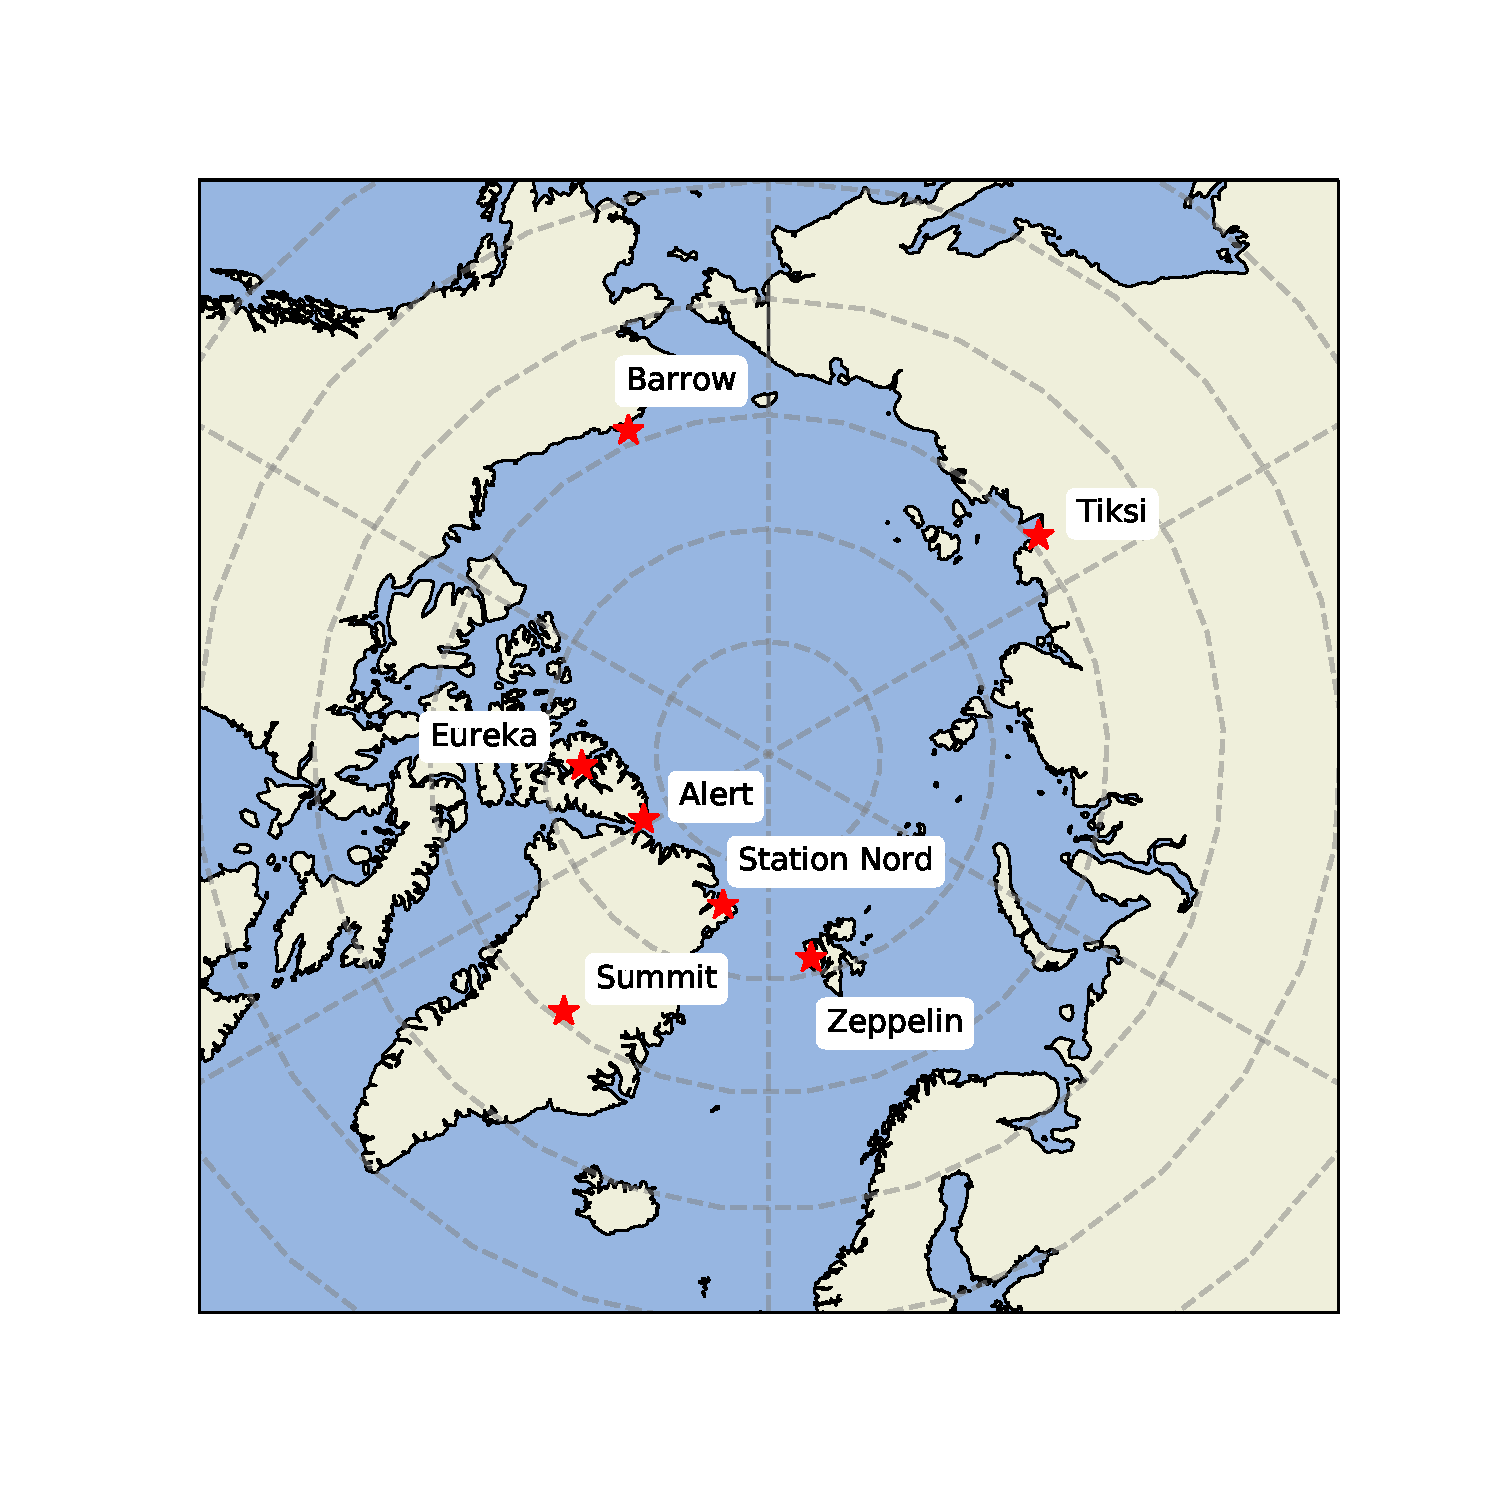
\includegraphics[width = .8\linewidth]{Chapter1_Intro/images/StationMap.pdf}
    \caption{Map of the stations used in comparison. Coordinates are listed in Table \ref{tab:stns}}
    \label{fig:stns}
\end{figure}
\begin{table}[h]
\centering
\resizebox{\columnwidth}{!}{%
\begin{tabular}{|llll|}
\hline
\textbf{Station}                 & \textbf{Location}       & \textbf{Altitude} & \textbf{Reference}     \\ \hline
Alert, Canada                    & 82$^o$50'N, 62$^o$34'W  & 210.0 m           & \cite{EBAS}, \cite{ESRL} \\
Barrow, Alaska, U.S.             & 71$^o$19'N, 156$^o$37'W & 11.0              & \cite{ESRL}            \\
Eureka, Canada                   & 80$^o$03'N, 86$^o$24'W  & 610.0 m           & \cite{EBAS}            \\
Station Nord, Greenland, Denmark & 81$^o$36'N, 16$^o$40'W  & 20.0 m            & \cite{EBAS}            \\
Summit, Greenland, Denmark       & 72$^o$34'N, 38$^o$28'W  & 3238.0 m          & \cite{EBAS}, \cite{ESRL} \\
Tiksi, Siberia, Russia           & 71$^o$58'N, 128$^o$92'E & 8.0 m             & \cite{EBAS}, \cite{ESRL} \\
Zeppelin, Svalbard, Norway       & 78$^o$54'N, 11$^o$53'E  & 474.0 m           & \cite{EBAS}            \\ \hline
\end{tabular}
}
\caption{Information about stations used in the comparison of model results and measured ozone}
\label{tab:stns}
\end{table}

\subsection{Code Availability}

The Oslo CTM3 v1.1 is available on GitHub at \url{https://github.com/NordicESMhub/OsloCTM3}. The developing branches I have used are called:

\begin{itemize}
    \item \texttt{marikoll\_originalCTM3\_NoStrat}: present day, original CTM3, no stratosphere 
    \item \texttt{marikoll\_originalCTM3\_noStrat\_pi}: pre-industrial, original CTM3, no stratosphere
    \item \texttt{marikoll\_bromine\_explosion\_susanne}: present day, halogen chemistry, no stratosphere
    \item \texttt{marikoll\_bromine\_explosion\_PI}: pre-industrial, halogen chemistry, no stratosphere
\end{itemize}


